%╔════════════════════════════╗
%║	  Szablon dostosował	  ║
%║	mgr inż. Dawid Kotlarski  ║
%║		  08.10.2023		  ║
%╚════════════════════════════╝
\documentclass[12pt,twoside,a4paper,openany]{article}

    % ------------------------------------------------------------------------
% PAKIETY
% ------------------------------------------------------------------------

%różne pakiety matematyczne, warto przejrzeć dokumentację, muszą być powyżej ustawień językowych.
\usepackage{mathrsfs}   %Różne symbole matematyczne opisane w katalogu ~\doc\latex\comprehensive. Zamienia \mathcal{L} ze zwykłego L na L-transformatę.
\usepackage{eucal}      %Różne symbole matematyczne.
\usepackage{amssymb}    %Różne symbole matematyczne.
\usepackage{amsmath}    %Dodatkowe funkcje matematyczne, np. polecenie \dfac{}{} skladajace ulamek w trybie wystawionym (porównaj $\dfrac{1}{2}$, a $\frac{1}{2}$).

%język polski i klawiatura
\usepackage[polish]{babel}
%\usepackage{qtimes} % czcionka Times new Roman
\usepackage[OT4]{polski}
%\usepackage[cp1250]{inputenc}                       %Strona kodowa polskich znaków.

%obsługa pdf'a
\usepackage[pdftex,usenames,dvipsnames]{color}      %Obsługa kolorów. Opcje usenames i dvipsnames wprowadzają dodatkowe nazwy kolorow.
\usepackage[pdftex,pagebackref=false,draft=false,pdfpagelabels=false,colorlinks=true,urlcolor=blue,linkcolor=black,citecolor=green,pdfstartview=FitH,pdfstartpage=1,pdfpagemode=UseOutlines,bookmarks=true,bookmarksopen=true,bookmarksopenlevel=2,bookmarksnumbered=true,pdfauthor={Dawid Kotlarski},pdftitle={Praca Inznierska},pdfsubject={},pdfkeywords={transient recovery voltage trv},unicode=true]{hyperref}   %Opcja pagebackref=true dotyczy bibliografii: pokazuje w spisie literatury numery stron, na których odwołano się do danej pozycji.

%bibliografia
%\usepackage[numbers,sort&compress]{natbib}  %Porządkuje zawartość odnośników do literatury, np. [2-4,6]. Musi być pod pdf'em, a styl bibliogfafii musi mieć nazwę z dodatkiem 'nat', np. \bibliographystyle{unsrtnat} (w kolejności cytowania).
\usepackage[
backend=biber,
style=numeric,
sorting=none
]{biblatex}
\addbibresource{bibliografia.bib}
\usepackage{hypernat}                       %Potrzebna pakietowi natbib do wspolpracy z pakietem hyperref (wazna kolejnosc: 1. hyperref, 2. natbib, 3. hypernat).

%grafika i geometria strony
\usepackage{extsizes}           %Dostepne inne rozmiary czcionek, np. 14 w poleceniu: \documentclass[14pt]{article}.
\usepackage[final]{graphicx}
\usepackage[a4paper,left=3.5cm,right=2.5cm,top=2.5cm,bottom=2.5cm]{geometry}

%strona tytułowa
\usepackage{strona_tytulowa}

%inne
\usepackage[hide]{todo}                     %Wprowadza polecenie \todo{treść}. Opcje pakietu: hide/show. Polecenie \todos ma byc na koncu dokumentu, wszystkie \todo{} po \todos sa ignorowane.
\usepackage[basic,physics]{circ}            %Wprowadza środowisko circuit do rysowania obwodów elektrycznych. Musi byc poniżej pakietow językowych.
\usepackage[sf,bf,outermarks]{titlesec}     %Troszczy się o wygląd tytułów rozdziałów (section, subsection, ...). sf oznacza czcionkę sans serif (typu arial), bf -- bold. U mnie: oddzielna linia dla naglowku paragraph. Patrz tez: tocloft -- lepiej robi format spisu tresci.
\usepackage{tocloft}                        %Troszczy się o format spisu trsci.
\usepackage{expdlist}    %Zmienia definicję środowiska description, daje większe możliwości wpływu na wygląd listy.
\usepackage{flafter}     %Wprowadza parametr [tb] do polecenia \suppressfloats[t] (polecenie to powoduje nie umieszczanie rysunkow, tabel itp. na stronach, na ktorych jest to polecenie (np. moze byc to stroma z tytulem rozdzialu, ktory chcemy zeby byl u samej gory, a nie np. pod rysunkiem)).
\usepackage{array}       %Ładniej drukuje tabelki (np. daje wiecej miejsca w komorkach -- nie są tak ścieśnione, jak bez tego pakietu).
\usepackage{listings}    %Listingi programow.
\usepackage[format=hang,labelsep=period,labelfont={bf,small},textfont=small]{caption}   %Formatuje podpisy pod rysunkami i tabelami. Parametr 'hang' powoduje wcięcie kolejnych linii podpisu na szerokosc nazwy podpisu, np. 'Rysunek 1.'.
\usepackage{appendix}    %Troszczy się o załączniki.
\usepackage{floatflt}    %Troszczy się o oblewanie rysunkow tekstem.
\usepackage{here}        %Wprowadza dodtkowy parametr umiejscowienia rysunków, tabel, itp.: H (duże). Umiejscawia obiekty ruchome dokladnie tam gdzie są w kodzie źródłowym dokumentu.
\usepackage{makeidx}     %Troszczy się o indeks (skorowidz).

%nieużywane, ale potencjalnie przydatne
\usepackage{sectsty}           %Formatuje nagłówki, np. żeby były kolorowe -- polecenie: \allsectionsfont{\color{Blue}}.
%\usepackage{version}           %Wersje dokumentu.

%============
\usepackage{longtable}			%tabelka
%============

%============
% Ustawienia listingów do kodu
%============

\usepackage{listings}
\usepackage{xcolor}

\definecolor{codegreen}{rgb}{0,0.6,0}
\definecolor{codegray}{rgb}{0.5,0.5,0.5}
\definecolor{codepurple}{rgb}{0.58,0,0.82}
\definecolor{backcolour}{rgb}{0.95,0.95,0.92}

% Definicja stylu "mystyle"
\lstdefinestyle{mystyle}{
	backgroundcolor=\color{backcolour},   
	commentstyle=\color{codegreen},
	keywordstyle=\color{blue},	%magenta
	numberstyle=\tiny\color{codegray},
	stringstyle=\color{codepurple},
	basicstyle=\ttfamily\footnotesize,
	breakatwhitespace=false,         
	breaklines=true,                 
	captionpos=b,                    
	keepspaces=true,                 
	numbers=left,                    
	numbersep=5pt,                  
	showspaces=false,                
	showstringspaces=false,
	showtabs=false,                  
	tabsize=2
}

\lstset{style=mystyle} % Deklaracja aktywnego stylu
%===========

%PAGINA GÓRNA I DOLNA
\usepackage{fancyhdr}          %Dodaje naglowki jakie się chce.
\pagestyle{fancy}
\fancyhf{}
% numery stron w paginie dolnej na srodku
\fancyfoot[C]{\scriptsize DOKUMENTACJA PROJEKTU - ZAAWANSOWANE PROGRAMOWANIE \\ 
\normalsize\sffamily  \thepage}


%\fancyhead[L]{\small\sffamily \nouppercase{\leftmark}}
\fancyhead[C]{\footnotesize \textit{AKADEMIA NAUK STOSOWANYCH W NOWYM SĄCZU}\\}

\renewcommand{\headrulewidth}{0.4pt}
\renewcommand{\footrulewidth}{0.4pt}

    % ------------------------------------------------------------------------
% USTAWIENIA
% ------------------------------------------------------------------------

% ------------------------------------------------------------------------
%   Kropki po numerach sekcji, podsekcji, itd.
%   Np. 1.2. Tytuł podrozdziału
% ------------------------------------------------------------------------
\makeatletter
    \def\numberline#1{\hb@xt@\@tempdima{#1.\hfil}}                      %kropki w spisie treści
    \renewcommand*\@seccntformat[1]{\csname the#1\endcsname.\enspace}   %kropki w treści dokumentu
\makeatother

% ------------------------------------------------------------------------
%   Numeracja równań, rysunków i tabel
%   Np.: (1.2), gdzie:
%   1 - numer sekcji, 2 - numer równania, rysunku, tabeli
%   Uwaga ogólna: o otoczeniu figure ma być najpierw \caption{}, potem \label{}, inaczej odnośnik nie działa!
% ------------------------------------------------------------------------
\makeatletter
    \@addtoreset{equation}{section} %resetuje licznik po rozpoczęciu nowej sekcji
    \renewcommand{\theequation}{{\thesection}.\@arabic\c@equation} %dodaje kropki

    \@addtoreset{figure}{section}
    \renewcommand{\thefigure}{{\thesection}.\@arabic\c@figure}

    \@addtoreset{table}{section}
    \renewcommand{\thetable}{{\thesection}.\@arabic\c@table}
\makeatother

% ------------------------------------------------------------------------
% Tablica
% ------------------------------------------------------------------------
\newenvironment{tabela}[3]
{
    \begin{table}[!htb]
    \centering
    \caption[#1]{#2}
    \vskip 9pt
    #3
}{
    \end{table}
}

% ------------------------------------------------------------------------
% Dostosowanie wyglądu pozycji listy \todos, np. zamiast 'p.' jest 'str.'
% ------------------------------------------------------------------------
\renewcommand{\todoitem}[2]{%
    \item \label{todo:\thetodo}%
    \ifx#1\todomark%
        \else\textbf{#1 }%
    \fi%
    (str.~\pageref{todopage:\thetodo})\ #2}
\renewcommand{\todoname}{Do zrobienia...}
\renewcommand{\todomark}{~uzupełnić}

% ------------------------------------------------------------------------
% Definicje
% ------------------------------------------------------------------------
\def\nonumsection#1{%
    \section*{#1}%
    \addcontentsline{toc}{section}{#1}%
    }
\def\nonumsubsection#1{%
    \subsection*{#1}%
    \addcontentsline{toc}{subsection}{#1}%
    }
\reversemarginpar %umieszcza notki po lewej stronie, czyli tam gdzie jest więcej miejsca
\def\notka#1{%
    \marginpar{\footnotesize{#1}}%
    }
\def\mathcal#1{%
    \mathscr{#1}%
    }
\newcommand{\atp}{ATP/EMTP} % Inaczej: \def\atp{ATP/EMTP}

% ------------------------------------------------------------------------
% Inne
% ------------------------------------------------------------------------
\frenchspacing                      
\hyphenation{ATP/-EMTP}             %dzielenie wyrazu w danym miejscu
\setlength{\parskip}{3pt}           %odstęp pomiędzy akapitami
\linespread{1.3}                    %odstęp pomiędzy liniami (interlinia)
\setcounter{tocdepth}{4}            %uwzględnianie w spisie treści czterech poziomów sekcji
\setcounter{secnumdepth}{4}         %numerowanie do czwartego poziomu sekcji 
\titleformat{\paragraph}[hang]      %wygląd nagłówków
{\normalfont\sffamily\bfseries}{\theparagraph}{1em}{}



    %polecenia zdefiniowane w pakiecie strona_tytulowa.sty
    \title{...Algorytm listy dwukierunkowej \\z zastosowaniem GitHub...}		%...Wpisać nazwę projektu...
    \author{Imie Nazwisko}
    \authorI{}
    \authorII{}		%jeśli są dwie osoby w projekcie to zostawiamy:    \authorII{}
		
	\uczelnia{AKADEMIA NAUK STOSOWANYCH \\W NOWYM SĄCZU}
    \instytut{Wydział Nauk Inżynieryjnych}
    \kierunek{Katedra Informatyki}
    \praca{DOKUMENTACJA PROJEKTOWA}
    \przedmiot{ZAAWANSOWANE PROGRAMOWANIE}
    \prowadzacy{mgr inż. Dawid Kotlarski}
    \rok{2023}


%definicja składni mikrotik
\usepackage{fancyvrb}
\DefineVerbatimEnvironment{MT}{Verbatim}%
{commandchars=\+\[\],fontsize=\small,formatcom=\color{red},frame=lines,baselinestretch=1,} 
\let\mt\verb 
%zakonczenie definicji składni mikrotik

\usepackage{fancyhdr}    %biblioteka do nagłówka i stopki

			
\begin{document}
   
    \renewcommand{\figurename}{Rys.}    %musi byc pod \begin{document}, bo w~tym miejscu pakiet 'babel' narzuca swoje ustawienia
    \renewcommand{\tablename}{Tab.}     %j.w.
    \thispagestyle{empty}               %na tej stronie: brak numeru
    \stronatytulowa                     %strona tytułowa tworzona przez pakiet strona_tytulowa.tex
 
 \pagestyle{fancy}

    \newpage

    %formatowanie spisu treści i~nagłówków
    \renewcommand{\cftbeforesecskip}{8pt}
    \renewcommand{\cftsecafterpnum}{\vskip 8pt}
    \renewcommand{\cftparskip}{3pt}
    \renewcommand{\cfttoctitlefont}{\Large\bfseries\sffamily}
    \renewcommand{\cftsecfont}{\bfseries\sffamily}
    \renewcommand{\cftsubsecfont}{\sffamily}
    \renewcommand{\cftsubsubsecfont}{\sffamily}
    \renewcommand{\cftparafont}{\sffamily}
    %koniec formatowania spisu treści i nagłówków
     
    \tableofcontents    %spis treści
    \thispagestyle{fancy}
    \newpage

    
    \newpage

    
%%%%%%%%%%%%%%%%%%% treść główna dokumentu %%%%%%%%%%%%%%%%%%%%%%%%%

   	\newpage
\section{Ogólne określenie wymagań}		%1
%Określenie celu pracy, co chcemy uzyskać, jakie przewidujemy wyniki













\hspace{0.60cm}Pierwszym celem projektu jest wykonanie programu listy dwukierunkowej opartej na stercie. Działanie listy ma zostać zaimplementowane w klasie oraz ma zawierać metody odpowiadające za:
\begin{itemize}
    \item Dodanie elementu na początku listy
    \item Dodanie elementu na końcu listy
    \item Dodanie elementu pod wskazany indeks
    \item Usunięcie elementu z początku listy
    \item Usunięcie elementu z końca listy
    \item Usunięcie elementu z pod wskazanego indeksu
    \item Wyświetlanie listy
    \item Wyświetalnie listy w odwrotnej kolejności
    \item Wyświetlanie nasępnego elementu
    \item Wyświetlanie poprzedniego elementu
    \item Czyszczenie całej listy
\end{itemize}
Działanie klasy i metody ma zostać przetestowane w funkcji main.

\hspace{0.60cm}Drugim celem projektu jest zapoznanie się z programem do kontroli wersji GitHub. Należy stworzyć na nim konto i zapisywać postępy nad projektem. Przy oddaniu projektu zaprezentować:
\begin{itemize}
    \item Co najmniej 5 commit'ów
    \item Co najmniej jedno cofnięcie się o dwa commit'y
    \item Usunięcie jednego commit'a
\end{itemize}

Listing kodu

\begin{lstlisting}[caption=Przykładowy kod 001, label={lst:listing-cpp}, language=C++]
#include <iostream>
#include <cstdlib>
#include <ctime>
using namespace std;

/*
liczby pseldolosowe
*/

int main(int argc, char** argv) {
	
	int tab[10][10];
	
	for(int i=0;i<10;i++)
	for(int j=0;j<10;j++)
	tab[i][j]=0;
	
	srand(time(NULL));		//generowanie z czasu
	int min=3;
	int max=7;
	for(int i=0;i<10;i++)
	for(int j=0;j<10;j++)		
	tab[i][j]=(rand()%(max-min+1))+min;	
	
	for(int i=0;i<10;i++)
	{
		for(int j=0;j<10;j++)
		cout<<tab[i][j]<<" ";	
		cout<<endl;
	}
	
	return 0;
}
\end{lstlisting}

Kod \ref{lst:listing-cpp} (s. \pageref{lst:listing-cpp}) przedstawia sposób generowania liczb pseudolosowych. Kod \ref{lst:listing-cpp2} (s. \pageref{lst:listing-cpp2}) przedstawia generowanie pliku HTML.

Alternatywna metoda wklejenia kodu:

\lstinputlisting[caption=Przykładowy kod 002, label={lst:listing-cpp2}, language=C++]{kod/main.cpp}
   \newpage
\section{Analiza problemu}		%2
%Napisać gdzie używa się tego algorytmu
%Opisać sposób działania programu/algorytmu
%Napisać spsoób wykorzystania algorytmu po przez wykonanie przykładu (np. mnożenie macierzy - wykonać ręcznie przykład z mnożeniem macierzy pokazujący jak mnoży się macierz ręcznie)
\hspace{0.60cm}Lista dwukierunkowa jest to struktura danych po której możemy poruszać się w dwóch kierunkach, do przodu i do tyłu. Każdy element zawiera wskaźnik na poprzedni (prev) lub następny (next) element w liście oraz dane (data) Rys. \ref{rys:rysunek001} (s. \pageref{rys:rysunek001}).

\begin{figure}[!htb]
	\begin{center}
		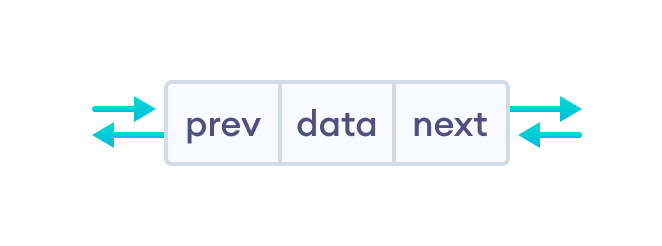
\includegraphics{Dokumentacja/rys/lista.png}
		\caption{Element listy.\footnotemark}
		\label{rys:rysunek001}
	\end{center}
\end{figure}

\footnotetext{\label{note1}Infografika ze strony https://www.programiz.com/dsa/doubly-linked-list\cite{www1}.}

\hspace{0.60cm}Na liście dwukierunkowej można przeprowadzać wiele operacji, takich jak dodawanie elementu na początek listy. Polega ono na połączeniu ze sobą wskaźnika next nowo stworzonego elementu ze wskaźnikiem prev elementu z początku listy (head) w taki sposób aby na siebie wskazywały Rys. \ref{rys:rysunek002} (s. \pageref{rys:rysunek002}).

\begin{figure}[!htb]
	\begin{center}
		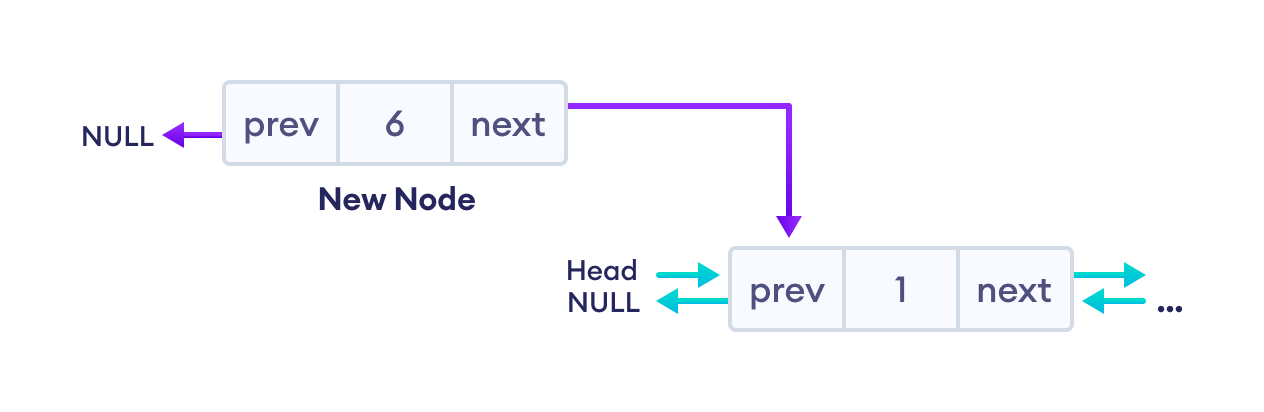
\includegraphics[scale=0.7]{Dokumentacja/rys/dodaj_na_poczatek.png}
		\caption{Dodawanie elementu na początek.\footref{note1}}
		\label{rys:rysunek002}
	\end{center}
\end{figure}

\newpage

\hspace{0.60cm}Kolejną operacją jest dodanie elementu na koniec. Przebiega ona podobnie jak z dodawaniem na początek z róźnicą, że łączymy ostatni element (tail) z nowo stworzonym Rys. \ref{rys:rysunek003} (s. \pageref{rys:rysunek003}).

\begin{figure}[!htb]
	\begin{center}
		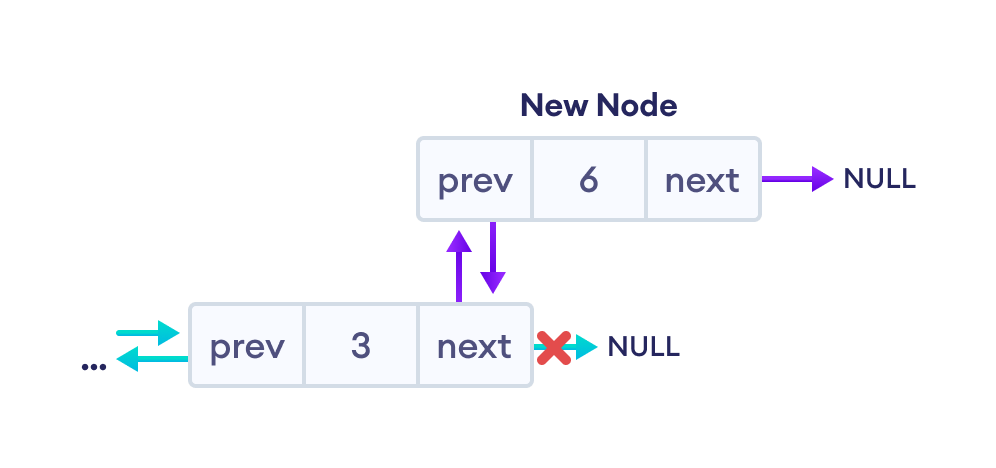
\includegraphics[scale=0.7]{Dokumentacja/rys/dodaj_na_koniec.png}
		\caption{Dodawanie elementu na koniec.\footref{note1}}
		\label{rys:rysunek003}
	\end{center}
\end{figure}

\footnotetext{\label{note1}Infografika ze strony https://www.programiz.com/dsa/doubly-linked-list\cite{www1}.}

\hspace{0.60cm}Możemy także wstawić element pod wskazany indeks łącząc ze sobą wskaźnik prev nowego elemnentu z wskaźnikiem next poprzedzającego indeks Rys. \ref{rys:rysunek004} (s. \pageref{rys:rysunek004}) oraz wskaźnik next z wskaźnikiem prev następnego po wskazanym indeksie Rys. \ref{rys:rysunek005} (s. \pageref{rys:rysunek005}).

\begin{figure}[!htb]
	\begin{center}
		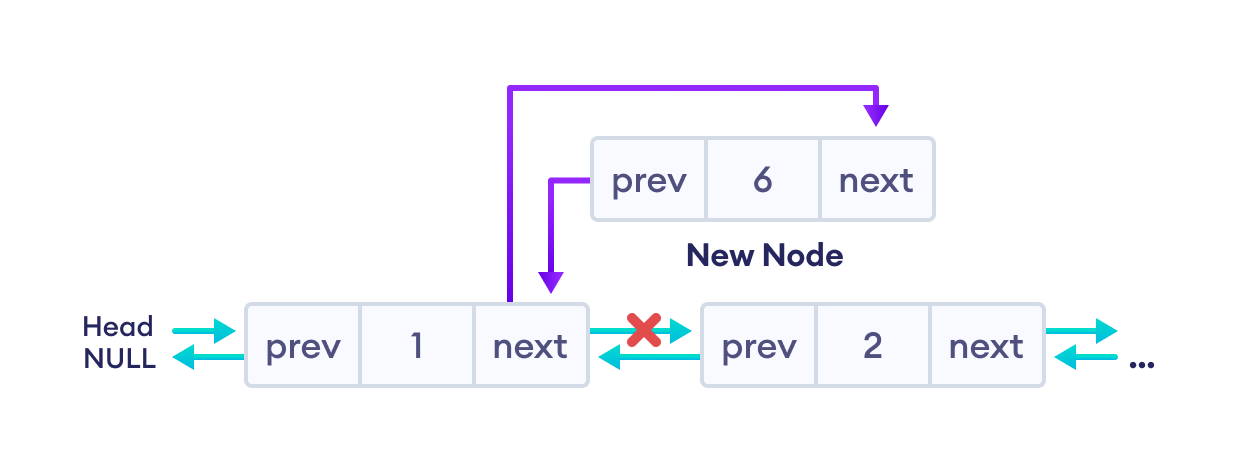
\includegraphics[scale=0.7]{Dokumentacja/rys/dodaj_indeks1.png}
		\caption{Łączenie z poprzedzającym elementem.\footref{note1}}
		\label{rys:rysunek004}
	\end{center}
\end{figure}

\newpage

\begin{figure}[!htb]
	\begin{center}
		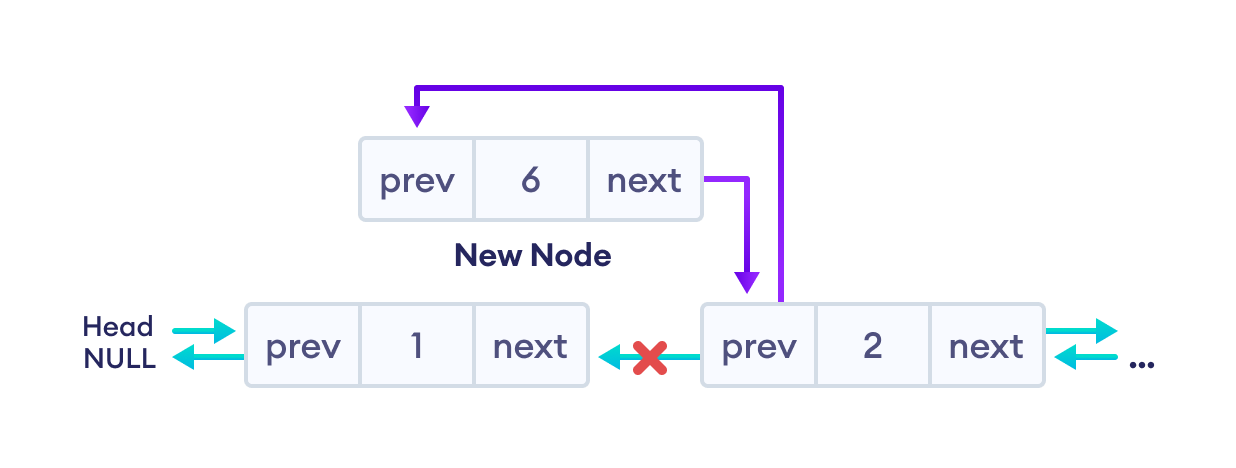
\includegraphics[scale=0.7]{Dokumentacja/rys/dodaj_indeks2.png}
		\caption{Łączenie z następnym elementem.\footref{note1}}
		\label{rys:rysunek005}
	\end{center}
\end{figure}

\footnotetext{\label{note1}Infografika ze strony https://www.programiz.com/dsa/doubly-linked-list\cite{www1}.}

\hspace{0.60cm}W analogiczny sposób przeprowadza się operację usuwania elementów z listy dwukierunkowej. Pierwszy i ostatni element usuwa się poprzez wpisywanie wartości NULL, żeby na nic nie wskazywały, do wskaźników elementów head i tail \ref{rys:rysunek006} i \ref{rys:rysunek007} (s. \pageref{rys:rysunek006}). Inaczej wygląda usuwanie wybranego elementu, gdzie łączy się ze sobą wskaźniki poprzedzającego i następującego elementu aby ten, którego chcemy się pozbyć nie należał już do listy \ref{rys:rysunek008} (s. \pageref{rys:rysunek008}).

\begin{figure}[!htb]
	\begin{center}
		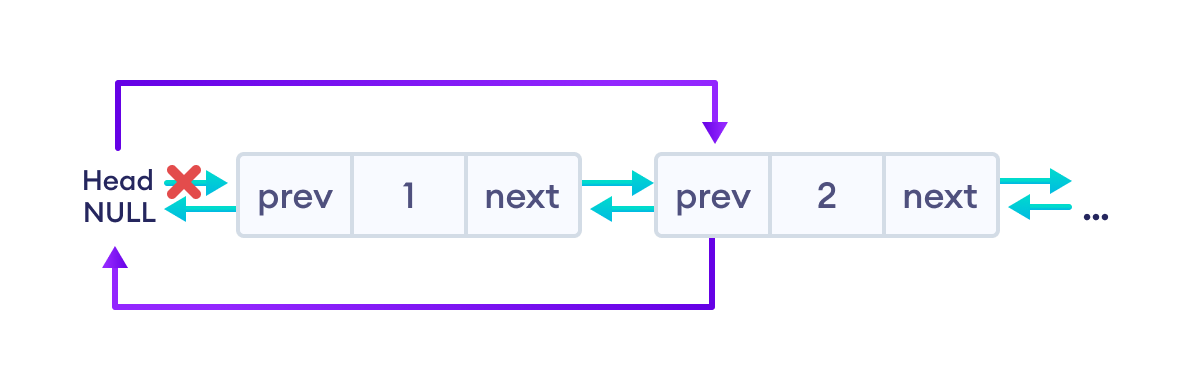
\includegraphics[scale=0.6]{Dokumentacja/rys/usun_przod.png}
		\caption{Usuwanie pierwszego elementu.\footref{note1}}
		\label{rys:rysunek006}
	\end{center}
\end{figure}

\begin{figure}[!htb]
	\begin{center}
		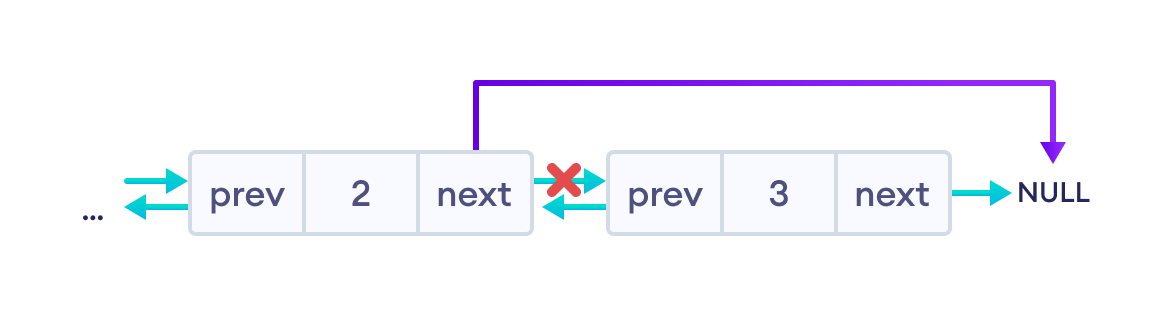
\includegraphics[scale=0.6]{Dokumentacja/rys/usun_koniec.png}
		\caption{Usuwanie ostatniego elementu.\footref{note1}}
		\label{rys:rysunek007}
	\end{center}
\end{figure}

\newpage

\footnotetext{\label{note1}Infografika ze strony https://www.programiz.com/dsa/doubly-linked-list\cite{www1}.}

\begin{figure}[!htb]
	\begin{center}
		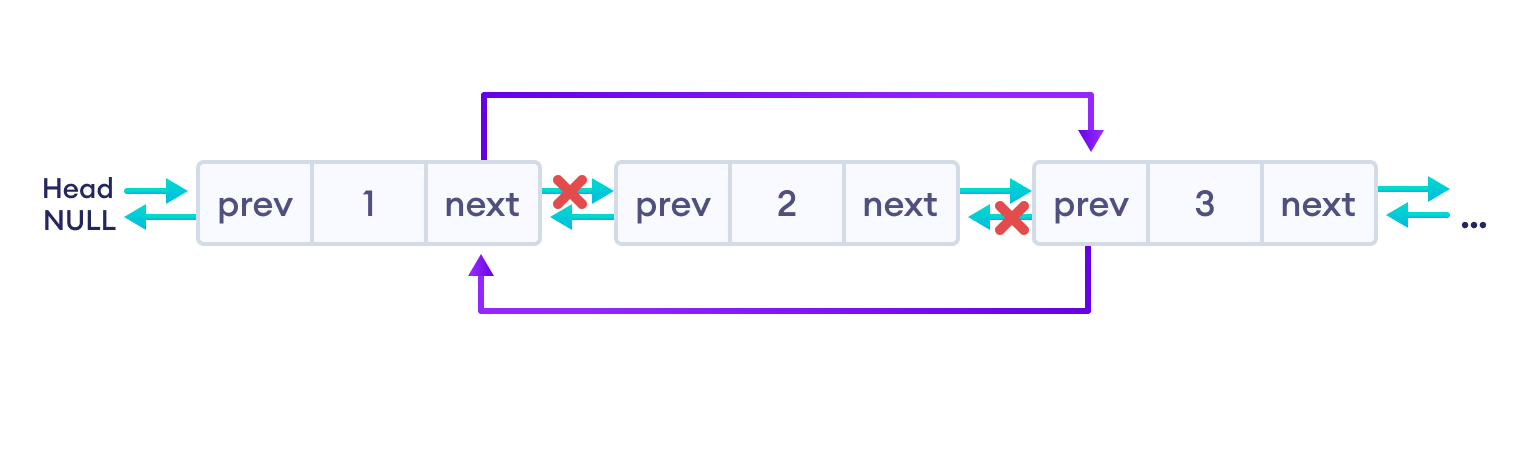
\includegraphics[scale=0.5]{Dokumentacja/rys/usun_srodek.png}
		\caption{Usuwanie wybranego elementu.\footref{note1}}
		\label{rys:rysunek008}
	\end{center}
\end{figure}

   	\newpage
\section{Projektowanie}		%3
%Napisać z jakich narzędzi będziemy korzystać (kompilator, język programowania), git, biblioteki dodatkowe, itp.
%Opisać szczegółowe ustawienia kompilatora (jeśli są), powiązania z bibliotekami, itp.
%Narysować graf, UML, diagram klas, schemat działania algorytmu




   	\newpage
\section{Implementacja}		%4
%Opisać implementacje algorytmu/programu. Pokazać ciekawe fragmenty kodu
%Opisać powstałe wyniki



   	\newpage
\section{Wnioski}	%5
%Npisać wnioski końcowe z przeprowadzonego projektu, 

\hspace{0.60cm}Tworzenie listy dwukierunkowej było bradzo ciekawym projektem, który byłem w stanie za pomocą znanych mi już narzędzi w języku C++ stworzyć. Dzięki niemu jestem w stanie sobie wyobrazić jak taka lista wygląda oraz w jaki sposób po niej się porusza. Nauczyłem się także używać bardzo przydatnego narzędzia do kotroli wersji znajdującego się na platformie GitHub\footnotemark.

\footnotetext{GitHub https://github.com\cite{www2}.}
   
       
%%%%%%%%%%%%%%%%%%% koniec treść główna dokumentu %%%%%%%%%%%%%%%%%%%%%
	\newpage
    \addcontentsline{toc}{section}{Literatura}  
	\printbibliography

    \newpage
    \hypersetup{linkcolor=black}
    \renewcommand{\cftparskip}{3pt}
    \clearpage
    \renewcommand{\cftloftitlefont}{\Large\bfseries\sffamily}
    \listoffigures
    \addcontentsline{toc}{section}{Spis rysunków}
	\thispagestyle{fancy}
	
    \newpage
    \renewcommand{\cftlottitlefont}{\Large\bfseries\sffamily}
    \def\listtablename{Spis tabel}
    \addcontentsline{toc}{section}{Spis tabel}\listoftables 
	\thispagestyle{fancy}
	
	\newpage
	\renewcommand{\cftlottitlefont}{\Large\bfseries\sffamily}
	\renewcommand\lstlistlistingname{Spis listingów}
	\addcontentsline{toc}{section}{Spis listingów}\lstlistoflistings 
	\thispagestyle{fancy}
	


    %lista rzeczy do zrobienia: wypisuje na koñcu dokumentu, patrz: pakiet todo.sty
    \todos
    %koniec listy rzeczy do zrobienia
\end{document}
